% -*- coding: utf-8; -*-

\chapter{Implementação da Compressão Horizontal}
\label{cap:impl_exp}

Esse capítulo apresenta a implementação do \textit{compressing}\footnote{\href{https://github.com/flavio-barros/compressing}{https://github.com/flavio-barros/compressing}}, compressor de provas que executa o algoritmo da Compressão Horizontal apresentado por Gordeev e Haeusler \cite{GordeevH16}. O objetivo desta implementação é fornecer os primeiros resultados empíricos da compressão e auxiliar na definição do algoritmo, aperfeiçoando procedimentos e estruturas de dados utilizadas durante o processo de compressão.

\section{Decisões de Projeto}

A finalização da formalização do algoritmo da Compressão Horizontal foi realizada paralelamente à implementação do \textit{compressing}, essa implementação tinha o objetivo inicial de retroalimentar a formalização do algoritmo com informações sobre a sua execução. Para gerar as informações sobre a execução do algoritmo seria necessário documentar os passos de execução através da geração de visualizações do grafo de prova durante o processo de compressão. Além da geração das visualizações, outro fator importante considerado durante a definição das decisões de projeto foi a necessidade de realizar várias modificações no código do compressor durante o desenvolvimento.

O \textit{compressing} foi implementado utilizando a linguagem de programação \textit{Python}. A escolha da linguagem levou em consideração a existência de uma implementação inicial da Compressão Horizontal escrita em Python, além de que a linguagem não demanda muito esforço para alterações no código e ainda possui várias bibliotecas com suporte a operações em grafos que possuem integração com o pacote de ferramentas de visualizações de grafos \textit{graphviz}.

\section{Estrutura do Projeto}

Utilizamos o padrão de projeto \textit{Adapter} para estruturar o projeto. A adoção do Adapter na estruturação do sistema permite a integração de classes externas ao sistema, convertendo a interface das classes externas à uma interface esperada pelas classes internas. 

A Figura \ref{fig:diag_adapter} mostra um exemplo de como as classes são estruturadas utilizando o \textit{Adapter}. Na \textit{Interface} são definidos os métodos que uma classe interna espera. A classe \textit{Adaptador} implementa a interface e utiliza os métodos da classe externa (\textit{ClasseAdaptada}) para definir os métodos esperados pela classe interna (\textit{ClasseCliente}).

\begin{figure}[ht]
  \begin{center}
    \fbox{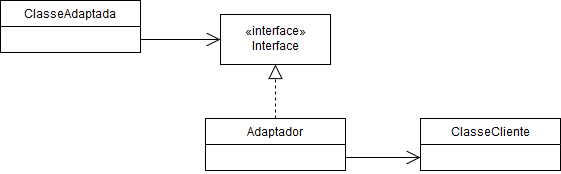
\includegraphics[height=80pt,width=257pt]{images/DiagramaClasse.png}}
    \caption{Exemplo de diagrama de classes do \textit{Adapter}}
    \label{fig:diag_adapter}
  \end{center}
\end{figure}

No \textit{compressing}, as classes adaptadas são dos pacotes que fornecem as funcionalidades de manipulação e visualização de grafos. A Figura \ref{fig:diag_comp} mostra o diagrama de classes simplificado do \textit{compressing}. A classe \textit{GraphAdapter} possui um objeto da classe \textit{DiGraph} e implementa a interface \textit{Graph}, que define todos os métodos de manipulação de grafos utilizados no \textit{compressing}. A implementação de cada método da classe \textit{GraphAdapter} adapta as funcionalidades oferecidas pela \textit{DiGraph}, que pertence ao pacote \textit{networkx}\footnote{\href{https://networkx.github.io/}{https://networkx.github.io/}}, para as funcionalidades definidas pela interface \textit{Graph}. A classe \textit{ProofGraph} implementa a EGDD definida na Seção \ref{sec:comp_hor} utilizando um objeto da classe \textit{GraphAdapter}. De maneira semelhante, a classe \textit{VisualGraphAdapter} converte as funcionalidades da classe \textit{Agraph}, do pacote pygraphviz\footnote{\href{https://pygraphviz.github.io/}{https://pygraphviz.github.io/}}, implementando os métodos definidos pela interface \textit{VisualGraph}. A principal diferença é que a \textit{VisualGraphAdapter} é utilizada por duas classes: a classe \textit{VisualProofGraph} implementa a visualização do do grafo de um objeto da \textit{ProofGraph}; a classe \textit{VisualCollapseGraph} implementa a geração da visualização de um colapso do processo de compressão, que é um subgrafo do grafo de um objeto da \textit{ProofGraph}.

\begin{figure}[ht]
  \begin{center}
    \fbox{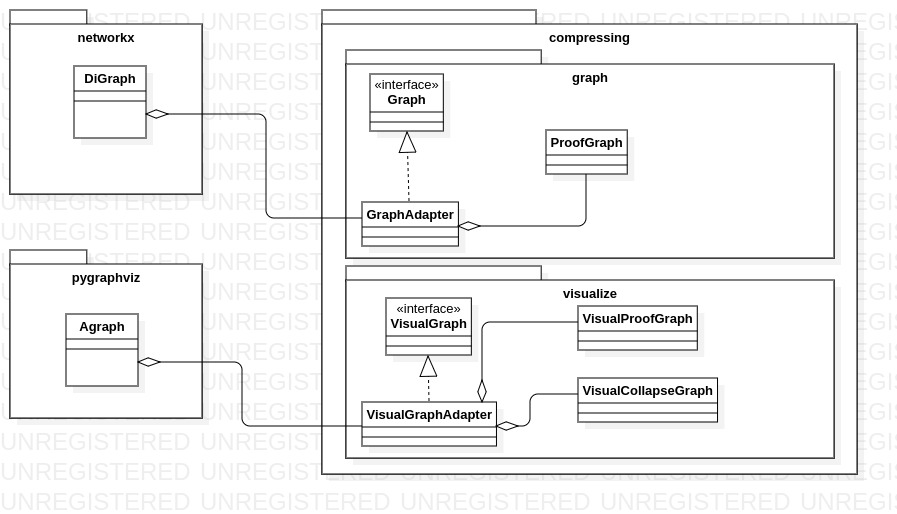
\includegraphics[height=230pt,width=400pt]{images/diagrama_classes.jpg}}
    \caption{Diagrama de classes simplificado do \textit{compressing}}
    \label{fig:diag_comp}
  \end{center}
\end{figure}

\section{Representação das Provas}

Os grafos de prova são representados por arquivos DOT, linguagem de descrição de grafos do \textit{graphviz}. A linguagem DOT pode representar grafos direcionados e não direcionados; subgrafos; atributos de grafos, vértices e arestas. O \textit{compressing} aceita somente arquivos \textit{.dot} que seguem as seguintes convenções:

\begin{itemize}
    \item Cada vértice do grafo é identificado por um \textit{id} e possui um atributo \textit{label}, que tem como valor a fórmula a qual o vértice é associado.
    \item Cada aresta de descarte possui um atributo \textit{comment} com o valor \textit{discharge}.
    \item As arestas dedutivas não possuem qualquer informação adicional.
\end{itemize}

Cada arquivo de saída possui as informações da EGDD adicionadas durante a compressão na forma de atributos de grafo, vértices e arestas. Cada arquivo gerado pelo \textit{compressing} segue as seguintes convenções:

\begin{itemize}
    \item A representação dos vértices é idêntica à dos arquivos de entrada.
    \item As arestas dedutivas que \textbf{não foram} colapsadas durante a compressão possuem três atributos: \textit{collapsed}, que possui valor \textit{False} indicando que a aresta não foi colapsada; \textit{color}, que possui como valor o numeral que indica sua cor; \textit{dependencies}, que possui como valor a cadeia de bits que indicam a dependência da fórmula do vértice que é sua origem.
    \item As arestas dedutivas que \textbf{foram} colapsadas durante a compressão possuem dois atributos: \textit{collapsed}, que possui valor \textit{True} indicando que a aresta foi colapsada; \textit{lambda-colors}, que possui como valor as cores das arestas dedutivas que a originaram.
    \item As arestas de ancestralidade possuem apenas um atributo, \textit{path}, que possui uma lista de cores que representa o caminho, através de arestas dedutivas, entre o vértice que é seu destino e o vértice que é a sua origem.
    \item O grafo possui um atributo, \textit{order}, que possui como valor a lista de fórmulas representando a ordenação linear utilizada para a construção das cadeias de bits de dependências.
\end{itemize}

